\documentclass{ctuthesis}
\ctusetup{
    xdoctype = B,
    xfaculty = F3,
    mainlanguage = english,
    titlelanguage = english,
    title-english = {Model of CAN FD Communication Controller for QEMU Emulator -- Analysis, Transmission and Reception},
    title-czech = {Model kontroléru CAN FD v emulátoru QEMU -- analýza, vysílání a příjem},
	doctype-english = {Bachelor Thesis},
    department-english = {Department of Control Engineering},
    author = {Jan Charvát},
	keywords-czech = {CAN bus, CAN FD, QEMU, Linux, CTU CAN FD, SocketCAN},
	keywords-english = {CAN bus, CAN FD, QEMU, Linux, CTU CAN FD, SocketCAN},
    supervisor = {Ing. Pavel Píša, Ph.D.},
    supervisor-address = {Praha 2\\ Karlovo náměstí 13\\ E-7a},
    month = 5,
    year = 2020,
}
\ctuprocess
\usepackage{tabularx, array, booktabs}
\begin{declaration}
Prohlašuji, že jsem předloženou práci vypracoval samostatně, a že jsem uvedl veškerou použitou literaturu.

V Praze, 17. ledna ~\ctufield{year}
\end{declaration}
\begin{thanks}
I would like to thank Ing. Pavel Píša Ph.D for tutoring and time investments towards my Thesis.
\end{thanks}
\begin{abstract-english}
 This thesis begins with a theoretical part, where is an analysis of CAN 2.0 and differences with newer standard CAN FD. It continues with QEMU CAN subsystem discovering. As a practical part is an implementation of CAN FD communication bus and emulation of CAN FD capable chip as an extension of already implemented CAN 2.0 capable chip SJA1000.
\end{abstract-english}

\begin{abstract-czech}
 Tato práce začíná teoretickou částí, kde je analýza CAN 2.0 a rozdíly s nevějším standardem CAN FD. Ta pokračuje s objevováním CAN subsystémů v QEMU. Jako praktická část je implementace CAN FD komunikační sběrnice a emulace čipu uzpůsobeného pro CAN FD jako rozšíření již implementovaného CAN 2.0 čipu SJA100.
\end{abstract-czech}

\begin{document}

\maketitle
\chapter*{Nomenclature}

\noindent
\begin{tabularx}{\linewidth}
  { l >{\raggedright\arraybackslash}X }
\bfseries Term & \bfseries Meaning \\\Midrule
CAN  & The angle of attack \\
ECU  & The real numbers \\
CAN & Controller Area Network \\
ECU & Electronic control unit \\
CANH & CAN-Hight line \\
CANL & CAN-Low line \\
SOF & Start of Frame \\
RTR & Remote request \\
IDE & Identifier Extension bit \\
DLC & Data Length Code \\
CRC & Cyclic redundancy check \\
ACK & Acknowledgement \\
\end{tabularx}

\chapter{Introduction}
 This bachelor thesis goal is to implement CAN FD communication bus and controller emulation for QEMU full system emulator mode. It builds on previous and ongoing CAN bus related projects developed and or coordinated by CTU FEE. The support of the classic SJA1000 CAN 2.0 controller model for QEMU emulator development started by Jin Yang in RTEMS GSoC 2013 slot mentored by Pavel Pisa from CTU and reached QEMU mainline in 2018. \cite{qemu-mainline} CTU CAN FD controller \cite{ctu-canfd-core} initiated by Ondrej Ille at CTU FEE is selected as the device model used by a guest system to access the CAN FD bus variant. Linux kernel driver for this controller is available as the result of Martin Jerabek's theses. \cite{ctu-canfd} \\
 The CAN controller core emulation needs to be connected to some system bus to be visible by emulated CPU and the guest system. The model of commercially available Kvaser PCI addon card is used for the SJA1000 emulation. The PCI Express card integration of CTU CAN FD is available as the project. \cite{ctu-project} \\
 SocketCan is used to interface QEMU emulated CAN bus to the CAN bus of the host system when QEMU is run on the Linux system. The QEMU side of the interface has to be extended to support CAN FD protocol.
 The most significant implementation part of this project is to emulate CTU CAN FD IP Core register map \cite{progdum} with QEMU and get communication through this emulated hardware parts on a real CAN hardware bus and see this communication on the other side by monitoring tools. \\
 This project is open-source the same as the whole QEMU. \\
 My focus to CAN bus is a result of participation in one external company
 project, which delivers utility for a train where CAN communication is used.

\chapter{CAN}
 Automotive industry often uses CAN.  For instance, almost every car uses CAN bus. One of the reasons is the need not to carry hundreds of kilograms of wire in the car. CAN enable the connection between several ECUs via one bus\cite{ECUs} instead of many analogue signal lines. Next advantage is that all nodes receive each message and decide if they want to use it or not. However, the application spectrum is broad. CAN standardised Bosch company in 1986. Hence make industry needs and CAN development significant progress. This bachelor thesis aim to the last most significant innovation CAN FD.

 \section{CAN 2.0}
  ISO 11898-1:2003 describes CAN 2.0. In the picture is a visible frame bit after bit. If it is to be sent 8 bytes data, it is visible a quite significant overhead. 
  \begin{figure}[H]
  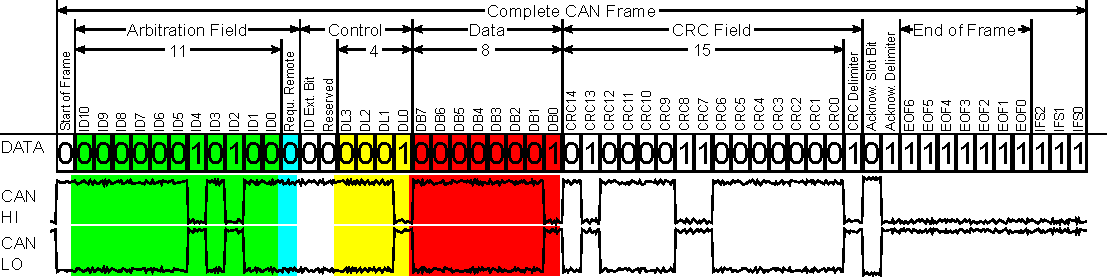
\includegraphics[width=1\textwidth]{CAN-Bus-frame_in_base_format_without_stuffbits}
  \caption{CAN frame detail \cite{can_frame}}
  \end{figure}
  The frame starts with SOF, which is always dominant zero. It serves to notify other CAN nodes at the beginning of the arbitration on the sending of a new frame. Then comes identifier, CAN 2.0 brings two length variants for ID, CAN 2.0a corresponds with a sample image and has an 11-bit identifier. CAN 2.0b standard extends identifier to 29-bit. RTR in dominant zero marks standard frame, in the recessive state it changes into a Remote frame, which requests for data from a CAN node with the corresponding ID assigned to the identifier place. IDE distinguished between standard and extended ID format. DLC holds data bytes count that is number between 0 to 8 bytes per message, then come the data. CRC is for data integrity check. ACK first bit is space for confirmation that at least one CAN node accept the message and the second bit for information that at least one CAN node has not accepted the message correctly. If the second condition is accomplished, the whole frame is resent automatically.
  \subsection{Physical layer}
   CAN physical layer consist of twisted pair cabling CANH and CANL. Logic value is counted as a result of CANH - CANL and is called Vd\cite{can_Vd}. Exact limiting values generally differ, but when both wires have similar voltage - Vd is close to zero, it is logic 1, and both wires are in recessive state. Dominant state means that in CANL decreased voltage and in CANH increased voltage, Vd gets over a specific limit into logic 0.
  \subsection{Transmission priority}
   CAN node priority depend on its ID, which must be unique across the bus. In the case, when more CAN nodes want to transmit data, arbitration wins the CAN node with the lowest ID. It means that can bus transmission is priority-based, and the highest priority is a CAN node with ID full of zeros. The reason comes from the physical layer, the transmission of the identifier is bitwise, and logical zero on the bus means a dominant state. Therefore, if the current's CAN node identifier contains 1, it wants to change the transmission to a recessive state. However, the dominant state representing a logical zero remains on the bus, the current CAN node realises that somewhere across the bus is also transmitting a CAN node with a higher priority, so this CAN node stops transmitting and switch to receive mode only and waits until next arbitration.
  \subsection{Bit stuffing}
   The final frame, which is sent through the bus, is not always fixed length because of the bit stuffing. This algorithm adds a different bit after five times repeated bit of same value. These redundant bytes relate to synchronisation algorithm because CAN bus does not have fixed timer authority. These bits could be added between SOF and the end of the  CRC and are not counted by CRC\cite{can_crc}.

 \section{CAN FD}
  CAN FD extends the original CAN with the flexible data rate, it means that data can have a higher bit rate than the rest of the frame. In CAN FD also increases maximum data length from 8 bytes to 64 bytes. All mentioned above describes ISO 11898-1:2015.
  \begin{figure}[H]
  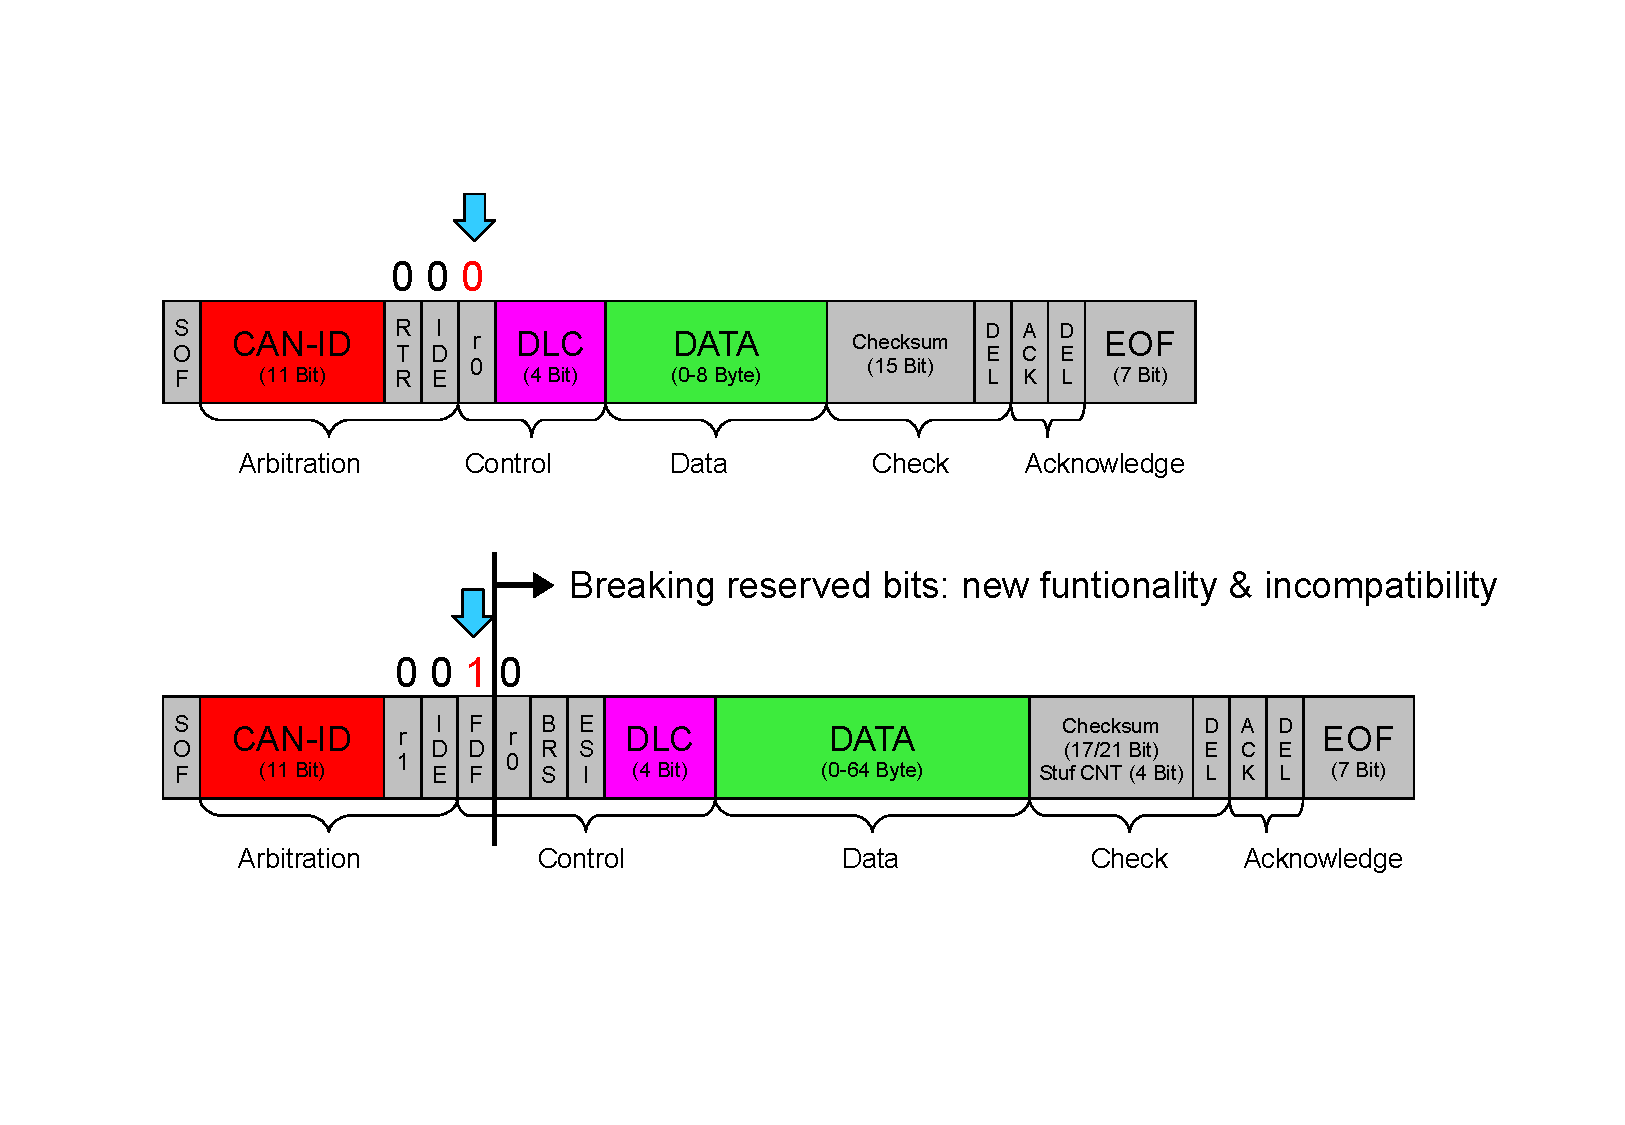
\includegraphics[width=1\textwidth]{agl2017-socketcan-can_fd}
  \caption{CAN and CAN FD difference \cite{canfd}}
  \end{figure}
  There is no direct compatibility between CAN and CAN FD due to flags as bit rate speed. Classic CAN would not recognize them and reject an error frame. Bit rate speed is 500 kbit/s for the arbitration phase and 2 Mbit/s or more for the data phase.
 
  \subsection{Data length code mapping}
   \begin{figure}[H]
   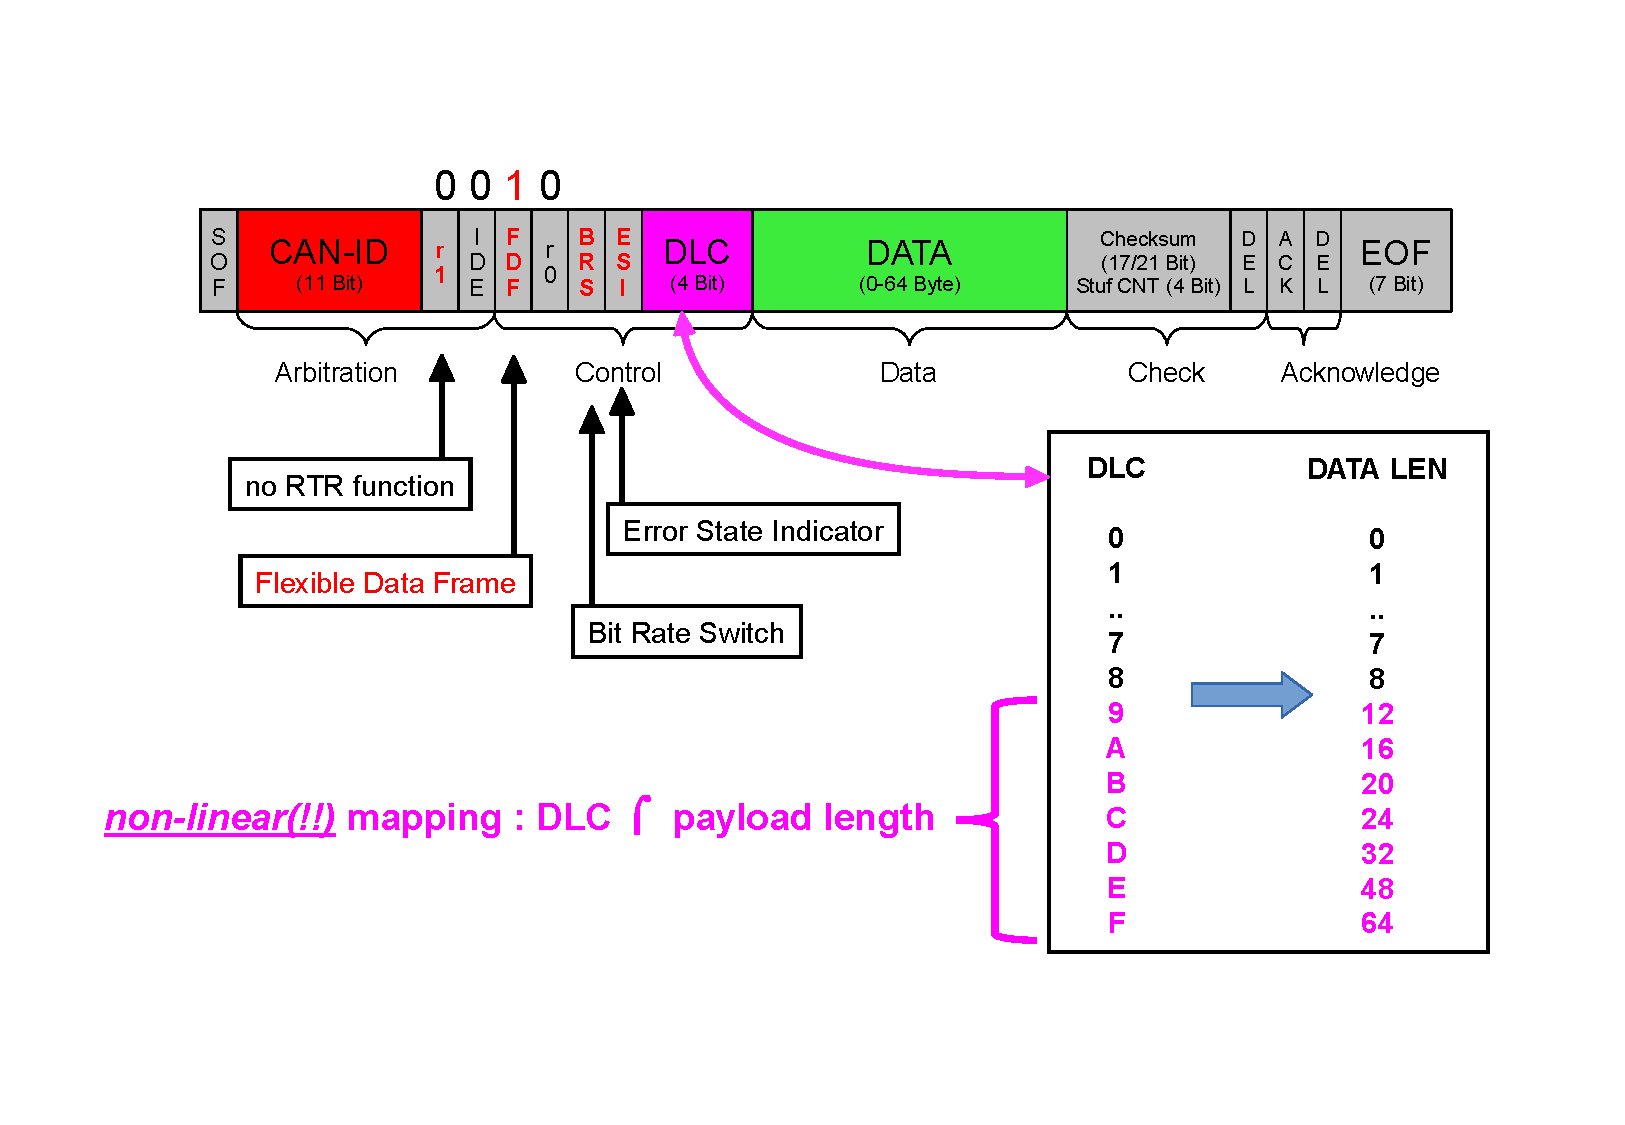
\includegraphics[width=1\textwidth]{agl2017-socketcan-can_fd_dlc}
   \caption{CAN FD frame DLC table \cite{canfd_dlc}}
   \end{figure}
   One of the most significant difference is a DLC flag which holds an individually coded length of the data. Data of arbitrary length up to 64 Bytes integrate into one of the possible intervals. First 8 Bytes correspond with standard CAN frames and continue with 12, 16, 20, 24, 32, 48 or 64 Bytes length.
 
\chapter{QEMU emulator}
 QEMU is a universal virtualisation tool because of several modes for working. The original purpose was to launch processes compiled for another architecture without the need to change current architecture (ARM, MIPS, Linux). However, it is used today more often for full system virtualisation including peripherals virtualisation. Support to CAN bus and controllers emulation has already been accepted into mainline. Nevertheless, CAN bus standard evolves, and a new extended variant of the protocol has been introduced in 2012. It is called CAN FD to highlight use of higher bit rate for the data portion of the frame.

 \section{Full system emulation}

 \section{QEMU architecture}
  Image bellow well describes emulation inside QEMU, and quite good explanation is in CAN support to QEMU emulator documentation. \cite[page 2-4]{qemu-mainline}
  \begin{figure}[H]
  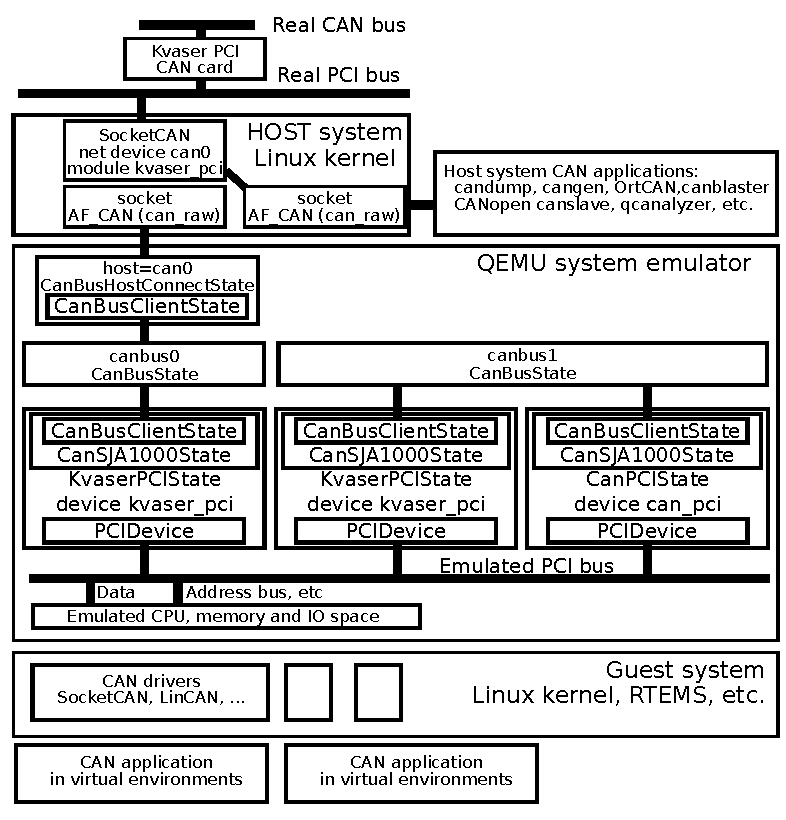
\includegraphics[width=1\textwidth]{qemu-can-bus}
  \caption{QEMU system emulator \cite{qemu-canbusexplain}}
  \end{figure}
  \section{Coding style}
 
 \section{QEMU subsystem}

 \section{Coding style}
  QEMU coding style \cite{qemu-style} is similar to the recommended Linux kernel style \cite{linux-style}. In QEMU repository is the script which checks the written code and shows all problems. The most common mistakes are tabs instead of 4 spaces, spaces or tabs on an empty line, wrong using of parenthesis.
 
\chapter{Implementation}
 
\section{Integration}

 \subsection{SocketCan support for CAN FD}
  Initial host SocketCan support has been added for CAN FD. SocketCan subsystem allows sending and receiving from the CAN controller. CAN FD frames handling requires to send structure with differences in memory size to SocketCan file handler. \\
  Struct qemu\_can\_frame has been extended to hold a longer data field and byte to store flags (BRS, etc.) has been defined. The frame is represented by the structure which contains ID with the unique 11 or extended 29 bits message identifier. A data buffer is increased from 8 bytes of CAN 2.0 to 64 bytes message of CAN FD.

 \subsection{CTU CAN FD core support}
  Initial CTU CAN FD core support has been started as a copy of SJA1000. Right at this moment is only SJA1000 chip controller supported. Therefore starts the creation of CTU controller supporting Can FD. \\
  When CTU CAN is integrated into a PCI Express board, then two BARs (Base Address Regions) are expected by the driver. The first keep value to identify the CAN core and provides a number of integrated core instances in the other region. The second region maps registers of the core instances one after another. The registers to control PCI Express MSI (Message Signaling Interrupts) and other FPGA chip-specific control functions are mapped at some offset to the first region as well. \\ 
  Add CTU CAN FD core register definitions by Ing. Ondrej Ille. It is a significant amount of memory mapping structures, precisely unions, which defines the layout of bits in real hardware. It distinguishes between several types of bits in hardware registers, read-only, write-only or read/write bits. Everything is in product documentation, and it is necessary to follow it for correct emulation behaviour.
 
 \subsection{Registers emulation}
  Initial implementation of TX buffers. Support of cyclic transmission buffers is necessary for correct message sending. Buffer stores whole frame inside and through interrupt requests for transmission. \\
  Add can\_dlc2len and can\_len2delc for CAN FD. These functions help with the conversion of DLC to standard LEN and the other way around. DLC uses an individual coding style precisely for this use case explain in CAN FD part.
  CAN FD and standard frames transmission. Last part of the implementation is to handle interrupts for transmission, Tx buffers state behaviour and implement less important read/write registers. \\
  The last step is to code clean up and more read-only registers.
 
  \subsubsection{Data structures}
 
 \subsection{Interrupts}
 
  \subsubsection{Interrupt mask}
  
  \subsubsection{Invoke interrupt}
 
 \subsection{SJA1000 CAN FD tolerant}

 \section{Transmission}

 \subsection{TX buffers}

  \subsubsection{Buffer states}
 
 \subsection{Commands}
 
 \subsection{Buffer to frame}
 
  \subsubsection{dlc to length}
 
 \section{Reception}

 \subsection{RX buffer}
 
  \subsubsection{FIFO implementation}
 
 \subsection{Commands}
 
 \subsection{Frame to buffer}
 
  \subsubsection{Length to dlc}
 
\chapter{Testing}
 Necessary commands to prepare the testing environment and check the functionality of written code if data go through, messages identifications correspond.
 \begin{verbatim}  cd mnt/shareddir/bin/
  cd ~/QEMU_PATH/shareddir/bin\end{verbatim}
 These are paths to shared memory for communication between inner and outer Linux systems during QEMU emulation. It is possible to add files or binaries into the emulated system during its run. The first one is a command of getting inside the emulated system to the right directory. The second one is the directory accessible from the outer system.
 \begin{verbatim}  modprobe ctucanfd_pci
  ip link set can1 type can bitrate 1000000 dbitrate 1000000 fd on
  ip link set can1 up
  cangen can1 -f\end{verbatim}
 Sequence for testing purpose. Load CTU CAN FD module into the Linux kernel, set up a virtual CAN interface and run
 \begin{verbatim}  ~/QEMU_PATH/scripts/checkpatch.pl ctucan_core.c\end{verbatim}
 Check script for correct code style.
 \begin{verbatim}  candump [can0]
  cangen  [can0]
          [-f] CAN FD frames\end{verbatim}
 Necessary tools to display, record, generate and test CAN traffic. \cite{can-utils}
 \begin{verbatim}  test-ctucan -p -T -I 0x123 -f -b\end{verbatim}
 Send CAN frame with additional settings and debug output.

 \section{Actual testing environment setup}
  This bachelor project develops on the system with Windows 10 where it runs utility for virtual machines VMware  Workstation 15 player in its free version in non-commercial use only. \cite{vmware} \\
  On VMware run virtual machine Ubuntu 18.04.3 LTS, \cite{ubuntu} inside Ubuntu take place whole work with QEMU. QEMU also use virtualisation, so during the work, for testing purpose, the next Linux system emulates inside the QEMU and results in virtualisation chain, which is not the best practice for working, but luckily, it is possible. In this case, QEMU uses the same build of the Linux kernel as an external system. It means Ubuntu 18.04.3 LTS. QEMU is possible to run with -nographic parameter, and it uses the current terminal window as its native console. \\

 \section{Test SW}
 
 \section{Driver}
 
\chapter{Conclusion}

 \section{Work already completed}
  This project analyses the basic QEMU concept and how to work with it as a full system emulator. Also shows proper coding style for QEMU.  Next part analyses CAN frames differences between standards to be able to understand which parts changed and how to implement them. It is necessary to know the role of each bit of CAN frame to be able to handle them. The analysis brings a group of often-used commands which helps with the workflow or with the testing.
 
 \subsection{Transmission and reception}

 \section{Implementation}
  Already working emulation of CAN bus and stand-alone SJA1000 controller support has been extended, CAN FD support has been added and now is CTUCAN FD core controller available with modified card CTUCAN PCI. Nowadays, the transmission of CAN FD frames is available. The new implementation keeps previous functionality of sending CAN 2.0 frames.

 \subsection{Future implementation goals}
  Consider messages rate slowdown as on real CAN bus. Some mechanism prevents to some limit lost of messages when a guest application is slow. Convert CAN bus model from plain C to QOM (Controllers are QOM/Qdev already). Add more CAN controllers model emulation (BOSCH/Ti C CAN, Freescale FlexCAN, etc.).
 
 \subsection{Transmission delay}
 
 \subsection{Vision}

\chapter{Attachment 1}
 
 \section{Installation guide for programmers}
  Check installation of git versioning system by
  \begin{verbatim}  git --version\end{verbatim}
  if there is no installation on computer write command
  \begin{verbatim}  sudo apt install git\end{verbatim}
  Now pull QEMU mainline from git
 \begin{verbatim}  git clone git://git.qemu.org/qemu.git\end{verbatim}
  Will continue with proper installation way. \\
  Until the project is not in mainline, it could be found here.
  \begin{verbatim}  git remote add gitlab-fel https://gitlab.fel.cvut.cz/canbus/qemu-canbus.git
   git checkout -b charvj10-canfd gitlab-fel/charvj10-canfd\end{verbatim}

\chapter{Attachment 2}

 \section{Useful commands}
  During the work is a great advantage to know some hidden features which are available on the actual system or program. It could make progress faster and simpler. A division between general Linux advice and specific testing purpose commands help with the problem understanding and shows personal usage what might do work easier.
 \section{Linux}
  For heavy Linux users are these commands and features natural, but for standard users, or mainly Windows programmers can help. The advice also contains shortcuts for Midnight Commander \cite{mc}. MC during the bachelor project proof itself as a great file explorer to browse and work with the file-system.
  \begin{verbatim}  F9 + cf\end{verbatim}
  MC F9 Command Find, go through the whole directory and try to find the written filename or keyword.
  \begin{verbatim}  lspci-full -v\end{verbatim}
  Display full information list about devices connected to the PCI bus.
  \begin{verbatim}  rdwrmem -b 4 -s 0x08010000 -l 100 -m\end{verbatim}
  Dump certain memory location. \cite{rdwrmem}
 
 
\renewcommand\bibname{References}
\begin{thebibliography}{1}
\bibitem{qemu-mainline} http://rtime.felk.cvut.cz/publications/public/rtlws2015-qemu-can.pdf
\bibitem{ctu-canfd-core} https://gitlab.fel.cvut.cz/canbus/ctucanfd\_ip\_core
\bibitem{ctu-canfd} https://dspace.cvut.cz/bitstream/handle/10467/80366/F3-DP-2019-Jerabek-Martin-Jerabek-thesis-2019-canfd.pdf
\bibitem{ctu-project} https://gitlab.fel.cvut.cz/canbus/pcie-ctu\_can\_fd
\bibitem{progdum} http://canbus.pages.fel.cvut.cz/ctucanfd\_ip\_core/Progdokum.pdf
\bibitem{qemu} https://help.ubuntu.com/lts/serverguide/qemu.html
\bibitem{vmware} https://www.vmware.com/products/workstation-player/workstation-player-evaluation.html
\bibitem{ubuntu} https://ubuntu.com/download/desktop
\bibitem{qemu-canbusexplain} https://www.linuxdays.cz/2017/video/Pavel\_Pisa-CAN\_canopen.pdf
\bibitem{qemu-style} https://github.com/portante/qemu/blob/master/CODING\_STYLE
\bibitem{linux-style} https://www.kernel.org/doc/html/v4.10/process/coding-style.html
\bibitem{ECUs} https://www.csselectronics.com/screen/page/simple-intro-to-can-bus/language/en
\bibitem{can_frame} https://upload.wikimedia.org/wikipedia/commons/5/5e/CAN-Bus-frame/\_in\_base\_format\_without\_stuffbits.svg
\bibitem{can_Vd} https://www.youtube.com/watch?v=YrJn2AyWVBc
\bibitem{can_crc} https://elearning.vector.com/mod/page/view.php?id=370
\bibitem{canfd} https://wiki.automotivelinux.org/\_media/agl-distro/agl2017-socketcan-print.pdf by Oliver Hartkopp - page 49
\bibitem{canfd_dlc} https://wiki.automotivelinux.org/\_media/agl-distro/agl2017-socketcan-print.pdf by Oliver Hartkopp - page 50
\bibitem{mc} https://midnight-commander.org/
\bibitem{rdwrmem} http://cmp.felk.cvut.cz/~pisa/linux/rdwrmem.c
\bibitem{can-utils} https://github.com/linux-can/can-utils/
\end{thebibliography}
\end{document}